\section{Algorithm}

In this section we describe the components of our algorithm and the
flow of data between these components.  The algorithm predicts the
syntactic category of a word in a given context based on its random
substitutes sampled from a statistical language model.  First, we
construct a pairwise co-occurrence representation of words and their
substitutes.  Next, we map each word and each substitute in the
co-occurrence data to real vectors (embeddings) on an $n$-dimensional
sphere using the S-CODE algorithm \cite{maron2010sphere}.  S-CODE
places the vectors for words that frequently co-occur with the same
substitutes (and substitutes that co-occur with the same words) close
to each other on the sphere.  We then apply k-means clustering to
group word and substitute embeddings and we induce word categories
from the resulting groups.  In Section~\ref{sec:cooc} we detail the
representation of words and their substitutes as co-occurrence data,
in Section~\ref{sec:embedding} we describe the embedding algorithm,
and finally in Section~\ref{sec:clustering} we describe the different
ways in which words and substitutes can be clustered to give us
categorizations of word types or tokens.


\subsection{Context Representation}
\label{sec:cooc}
% How we represent the context?
% How we relate the word and the context?

We represent the context of a word with random substitutes that are
likely to occupy the same position as the word.  We sample random
substitutes (with replacement) from a substitute word distribution for
the context calculated based on an n-gram language model.  The sample
space of the substitute word distribution is the vocabulary of the
language model.
%% \footnote{Sampled substitutes might include the unknown
%%   word tag \unk\ representing words outside the fixed size
%%   vocabulary of the language model.  For example proper nouns
%%   typically have \unk\ as a substitute.}  
In effect, we are using
substitute word distributions and the sampled random substitutes as
{\em contextual features} that represent properties of a word's
position.  Table~\ref{tab:subdist} shows the substitute word
distributions for some positions in an example sentence.

\begin{table}[h]
\caption{The substitute word distributions (with probabilities in
  parentheses) for some of the positions in the example sentence
  \textit{``Pierre Vinken, 61 years old, will join the board as a
    nonexecutive director Nov.~29.''} based on a 4-gram language
  model.}
\label{tab:subdist}
\begin{tabular}{|ll|} \hline
\textbf{will:} & \textit{will} (0.9985), \textit{would} (0.0007), \textit{to} (0.0006), \textit{also} (0.0001), $\ldots$ \\
\textbf{join:} & \textit{join} (0.6528), \textit{leave} (0.2140), \textit{oversee} (0.0559), \textit{head} (0.0262), \textit{rejoin} (0.0074), $\ldots$ \\
\textbf{the:}  &\textit{its} (0.9011), \textit{the} (0.0981), \textit{a} (0.0006), $\ldots$ \\
\textbf{board:} & \textit{board} (0.4288), \textit{company} (0.2584), \textit{firm} (0.2024), \textit{bank} (0.0731), \textit{strike} (0.0030), $\ldots$ \\
\hline
\end{tabular}
\end{table}

To capture the relation between each word and its context we construct
a co-occurrence representation by pairing the words with randomly
sampled substitutes.  Table~\ref{tab:samples} shows random substitutes
of each word and their pairwise co-occurrence representation input to
S-CODE for an example sentence.  It is possible (and beneficial) to
sample more than one substitute and generate multiple pairs for the
same word-context pair as seen in Table~\ref{tab:samples}.  A target
word might appear both as a word and a random substitute therefore to
clarify this ambiguity we prepend ``W:'' and ``S:'' to words and
substitutes, respectively, in the co-occurrence data.  The calculation
of substitute distributions and random substitute sampling are
detailed in Appendix~A.

\begin{table}[ht]
  \caption{The table on the left shows three possible substitutes
    sampled with replacement for each position in an example sentence
    based on a 4-gram language model.  The table on the right is the
    pairwise co-occurrence data fed to the S-CODE algorithm derived
    from these samples.  The prefixes ``W:'' and ``S:'' are used to
    distinguish target words and substitutes.  Sampled substitutes
    might include the unknown word tag ``\unk'' representing words
    outside the fixed size vocabulary of the language model.}
\begin{tabular}{|ll|} \hline
\textbf{Word} & \textbf{Random Substitutes}\\
\hline
Pierre & \textit{Mr.}  / \textit{Pierre} /  \textit{John}\\
Vinken & \textit{\unk} / \textit{Beregovoy} / \textit{Cardin}\\
, & \textit{,} / \textit{,} / \textit{,}\\
61 & \textit{48} / \textit{52} / \textit{41}\\
years & \textit{years} /  \textit{years} /  \textit{years}\\
old & \textit{old} /  \textit{old} /  \textit{old}\\
, & \textit{,} /  \textit{,} /  \textit{,}\\
will & \textit{will} /  \textit{will} /  \textit{will}\\
join & \textit{head} /  \textit{join} /  \textit{leave}\\
the  & \textit{its} /  \textit{its} /  \textit{the}\\
board & \textit{board} /  \textit{company} / \textit{firm}\\
as & \textit{as} / \textit{as} / \textit{as}\\
a & \textit{a} / \textit{a} / \textit{a}\\
nonexecutive & \textit{nonexecutive} / \textit{non-executive} / \textit{nonexecutive}\\
director & \textit{chairman} / \textit{chairman} / \textit{director}\\
Nov. & \textit{April} / \textit{May} / \textit{of}\\
29 & \textit{16} /  \textit{29} / \textit{9}\\
. & \textit{.}  / \textit{.} / \textit{.}\\
\hline
\end{tabular}
\quad
\begin{tabular}{|ll|}
\hline
\textbf{Word} & \textbf{Substitute}\\
\hline
W:Pierre & \textit{S:Mr.}\\
W:Pierre & \textit{S:Pierre}\\
W:Pierre & \textit{S:John}\\
W:Vinken & \textit{S:\unk}\\
W:Vinken & \textit{S:Beregovoy}\\
W:Vinken & \textit{S:Cardin}\\
$\hdots$&\\
W:join & \textit{S:head}\\
W:join & \textit{S:join}\\
W:join & \textit{S:leave}\\
W:the & \textit{S:its}\\
W:the & \textit{S:its}\\
W:the & \textit{S:the}\\
$\hdots$&\\
W:director & \textit{S:chairman}\\
W:director & \textit{S:chairman}\\
W:director & \textit{S:director}\\
$\hdots$&\\
\hline
\end{tabular}
\label{tab:samples}
\end{table}

The next section describes the S-CODE algorithm which takes the
pairwise co-occurrence data as its input and calculates the embeddings
of the words and their substitutes on an $n$-dimensional sphere.

\subsection{Co-occurrence Embedding}
\label{sec:embedding}
The S-CODE algorithm maps each unique word and substitute in the
co-occurrence data to a real vector (embedding) on an $n$-dimensional
sphere as detailed in Appendix~B.  The basic idea of the mapping is
that words and substitutes that are frequently observed as pairs in
the co-occurrence data will have close embeddings while pairs
not observed together will have embeddings that are far apart from each
other.

\begin{figure}[ht]
\centering
  \begin{minipage}[c]{0.38\textwidth}
    \begin{tabular}{|l|l|}
    \hline
    \textbf{Word} & \textbf{Substitute} \\
    \hline
    $\hdots$&$\hdots$\\
    W:director & S:chairman \\
    W:chief & S:chairman \\
    $\hdots$&$\hdots$\\
    W:Pierre & S:John \\
    W:Frank & S:John \\
    $\hdots$&$\hdots$\\
    \hline
  \end{tabular}
  \end{minipage}
  \begin{minipage}[c]{0.48\textwidth}
    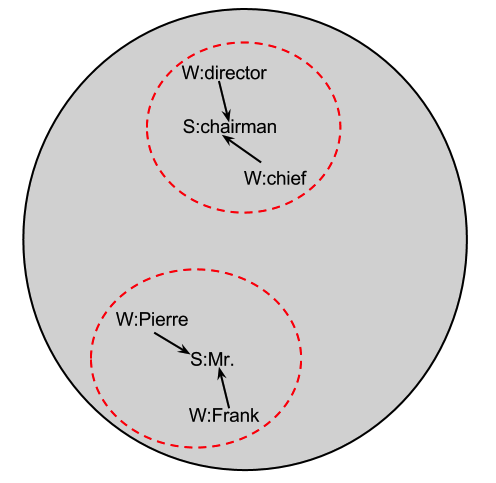
\includegraphics[height=.6\textwidth]{scode-ex.png}
  \end{minipage}
  \caption{The figure on the right represents the final embeddings for the
    words and substitutes from the co-occurrence data on the left after
    S-CODE converges.  Dashed circles represent the possible groupings
    of the embeddings on the sphere.}
  \label{fig:scodeexample}
\end{figure}

The co-occurrence data in Figure~\ref{fig:scodeexample} consists of
pairs such as (\textit{W:director}, \textit{S:chairman}) and
(\textit{W:chief}, \textit{S:chairman}) therefore S-CODE forces the
embeddings of \textit{W:director} and \textit{W:chief} to be close to
the embedding of \textit{S:chairman}.  Similarly the embeddings of
\textit{W:Pierre} and \textit{W:Frank} will be close to the embedding
of \textit{S:John} because they are frequently co-occurring pairs.  As
a result the final embeddings of \textit{W:director} and
\textit{W:chief} will be close to each other due to the common
substitute \textit{S:chairman} and will be apart from
\textit{W:Pierre} and \textit{W:Frank} due to the lack of common
substitutes (similarly the embeddings of \textit{W:Pierre} and
\textit{W:Frank} will be close to each other due to \textit{S:John}).

The coordinates of the embeddings for each unique word and substitute
constitute the input to the clustering stage as described in the next
subsection.

% How we relate final embeddings and the input pairs?
%% S-CODE constructs embeddings on an $n$-dimensional sphere for each word
%% type and substitute.  Each pair in the co-occurrence data can be
%% represented in three different ways by using the output of S-CODE: (1)
%% word embedding (${\bf W}$) which represents the word type information,
%% (2) substitute embedding (${\bf C}$) which represents the context
%% information, and (3) concatenation of word and substitute embeddings
%% (${\bf W}\oplus{\bf C}$).  In the next section we apply k-means
%% clustering to these three representation and analyze the
%% characteristic of final clusters.

\subsection{Clustering}
\label{sec:clustering}
%% In Section~\ref{sec:cooc} we describe the transformation of an input
%% sentence to a co-occurrence data and we represent each target word
%% with the word--substitute pair(s).  In the previous section we
%% construct embeddings for each value observed in the co-occurrence data
%% using the S-CODE algorithm. 

At this stage, each unique word in the text and each unique substitute
sampled to represent their contexts is mapped to a real vector
embedding on an $n$ dimensional sphere\footnote{In fact many words
  that appear in the text also appear as substitutes and thus get two
  embeddings.}.  We apply the instance weighted k-means clustering
algorithm to three different representations derived from these
embeddings, each with its own advantages and disadvantages:

\paragraph{Clustering word embeddings (${\bf W}$)} In the first setting,
we ignore substitute embeddings and apply clustering only to target
word embeddings.  Each target word {\em type} has a single embedding,
and gets assigned to a single cluster.  Thus clustering target words
based on this representation can only assign a single tag to each word
type and cannot represent multiple parts of speech for ambiguous
words (words that have more than one tag).  

For example, the word {\em offer} is tagged as NN(399), VB(105) and
VBP(34) in its 538 PTB occurrences\footnote{NN, VB and VBP are three
  part-of-speech tags from the Penn Treebank corpus and they
  correspond to singular noun, verb in base form and
  non-$3^{rd}$person singular verb in present tense, respectively.}.
When all instances of {\em offer} are assigned to the same cluster,
the \mto\ upper bound of {\em offer} will be 399/538=.74 using the
most frequent tag NN.

Clustering word embeddings was previously explored in
\cite{yatbaz-sert-yuret:2012:EMNLP-CoNLL}, which achieved the best
results to date (80\% \mto) for English.
Sections~\ref{sec:clustering-w} and \ref{sec:feat} summarize these
experiments for completeness.  The surprising success of the
one-tag-per-word assumption in English part of speech induction is
partly due to the fact that 93.69\% of the word occurrences in the
human labeled PTB data are tagged with their most frequent part of
speech \cite{Toutanova:2003:FPT:1073445.1073478}.  However the
clustering performance on ambiguous words is bounded and the utility
of a part of speech induction model which cannot handle ambiguity is
questionable.

%offer tag distribution in WSJ VBP 34, VB 105, NN 399
\paragraph{Clustering substitute embeddings (${\bf S}$)}  
In a second set of experiments, we ignore target word embeddings and
apply clustering only to substitute embeddings, associating each
substitute with a unique cluster.  We then categorize target word {\em
  tokens} based on what cluster the majority of their substitutes
belong.  It is important to note that in this setting we are ignoring
the identity and features of the target words and in effect clustering
word contexts (substitutes are determined by the context and are
conditionally independent of the target word).

For example, the target word {\it W:board} in Table~\ref{tab:samples}
will be represented with the embeddings of {\it S:board}, {\it
  S:company} and {\it S:firm} while another occurrence of the word
{\it W:board} in a different context might be represented with
embeddings of different substitutes such as {\it S:embark} or {\it
  S:enter}.  Each occurrence of the target word ``board'' is assigned
to the cluster in which the majority of its substitute embeddings are
present\footnote{Ties are broken randomly.}.  This approach generally
results in higher accuracy for highly ambiguous words like {\em offer}
where clustering substitute embeddings achieves .82 \mto\ compared
to the one-tag-per-word upper bound of .74.
Section~\ref{sec:clustering-s} presents the results of experiments
clustering substitute embeddings.

Unfortunately such highly ambiguous words do not constitute a
significant portion of the corpus and the overall accuracy suffers
(.64 compared to .80 \mto\ for word clustering).  We also observed
similar results in our preliminary experiments without S-CODE trying
to cluster contexts directly (using the Kullback-Leibler divergence
between their substitute distributions).  Many common words that occur
in similar contexts and that have similar substitutes, e.g. {\em his}
and {\em the}, belong to different parts of speech.  In addition,
words that are generally not substitutable like ``do'' and ``put'' are
placed in the same category by the PTB.  This suggests that the
identity and features of the target word are indispensable and that a
purely substitutability based linguistic definition is insufficient
for inducing parts of speech as tagged in the PTB.

\paragraph{Clustering the concatenation of word and substitute 
embeddings (${\bf W\oplus S}$)} In a third set of experiments we
concatenate the $n$-dimensional embedding vector for each sampled
substitute with the $n$-dimensional embedding vector of its target
word and apply clustering to the resulting $2n$-dimensional vectors.
We then categorize target word {\em tokens} based on what cluster the
majority of their substitute-concatenated vectors belong.  For
instance, the target word ``Pierre'' in Table~\ref{tab:samples} will
be represented with three vectors that will be the concatenation of
the embedding of {\it W:Pierre} with the embeddings of {\it S:Mr.},
{\it S:Pierre} and {\it S:John}, separately.  Models that are based on
this representation do not employ the one-tag-per-word assumption,
they can cluster word tokens, and they can represent ambiguity.
Clusters that are constructed according to this representation tend to
assign fewer categories to each word type than substitute clustering due to
the concatenation of ${\bf W}$.  The advantage in highly ambiguous
words is still retained (e.g. the \mto\ for {\em offer} is .89) and
the overall result is significantly improved (.70 \mto) compared to
substitute clustering.
Section~\ref{sec:clustering-concatenation} presents our experiments
clustering concatenated word-substitute vectors.

\paragraph{Summary} The first setting applies the one-tag-per-word
assumption from the beginning and clusters word types instead of
tokens.  The second setting clusters word contexts (as represented by
substitutes) and is able to categorize individual word tokens.
However it ignores the identity of the target word.  The third setting
also clusters word tokens but represents each token with a set of
concatenated word and substitute embeddings.  Representing the
identity of the target word without enforcing the one-tag-per-word
assumption improves the results on highly ambiguous words.
Section~\ref{sec:exp} compares the performance of these three settings
on the part of speech induction problem, as well as experiments with
different features and languages.
